\section{Metodología de Análisis de Factibilidad}

Aunque los modelos teóricos abundan en la literatura satelital, su aplicación efectiva exige una adaptación cuidadosa al contexto específico. Resulta revelador observar cómo la brecha entre simulaciones ideales y condiciones reales de operación determina el éxito o fracaso de proyectos como el VENESAT-2.

\subsection{Balance de enlace y simulaciones}

Uno de los pilares centrales de este estudio consiste en evaluar rigurosamente el desempeño del enlace bajo escenarios variados. Se adoptó un enfoque de balance de enlace determinístico y probabilístico que incorpora tanto condiciones nominales como degradadas.

La ecuación fundamental de balance de enlace empleada sigue la forma estándar adaptada para sistemas GEO en bandas Ku/Ka:

\begin{equation}
\left( \frac{C}{N_0} \right) = EIRP + G/T - L_{FS} - L_{atm} - L_{other} + k
\label{eq:link_budget}
\end{equation}

donde \(EIRP\) representa la potencia isotrópica radiada efectiva, \(G/T\) la figura de mérito de la estación receptora, \(L_{FS}\) la pérdida en espacio libre, \(L_{atm}\) las pérdidas atmosféricas (principalmente por lluvia) y \(k\) la constante de Boltzmann. 

Estudios previos sobre evaluación de desempeño en sistemas satelitales destacan la utilidad de este tipo de análisis para predecir márgenes operativos realistas \cite{LinkBudgetAnalysis2022}. En este trabajo se realizaron miles de simulaciones iterativas variando parámetros atmosféricos, elevación de antena y configuraciones redundantes.

\begin{table}[h]
\centering
\caption{Parámetros principales de simulación}
\label{tab:parametros_sim}
\begin{tabular}{lc}
\hline
\textbf{Parámetro} & \textbf{Valor / Rango} \\
\hline
Frecuencia (Ku/Ka) & 12/20 GHz \\
Potencia de saturación TWTA & 150 W \\
Diámetro antena terrena & 4.5 -- 7.2 m \\
Tasa de lluvia (0.01\%) & 20 -- 120 mm/h \\
Elevación mínima & 15° -- 65° \\
Márgenes de implementación & 2.5 dB \\
Iteraciones Monte Carlo & 10.000 \\
\hline
\end{tabular}
\end{table}

La Tabla 4 detalla los valores clave utilizados. Se implementaron scripts en Python/MATLAB para automatizar el cálculo de disponibilidad anual y generar curvas de excedencia.

\subsection{Análisis de confiabilidad FMEA}

Lejos de limitarse a métricas de enlace, la factibilidad operativa exige un examen profundo de la confiabilidad del sistema completo. Se aplicó la metodología FMEA de manera estructurada, siguiendo recomendaciones aeroespaciales adaptadas al contexto del proyecto.

Cada componente —desde el segmento espacial hasta las estaciones terrenas redundantes y los protocolos de conmutación— fue desglosado en modos de fallo potenciales. Se asignaron puntuaciones de severidad, ocurrencia y detectabilidad para calcular el Número de Prioridad de Riesgo (RPN). Este proceso permitió identificar los puntos críticos donde la redundancia 1+1 aporta mayor valor.

Particularmente instructivo resultó el cruce entre resultados FMEA y los balances de enlace. Configuraciones que parecían robustas sobre el papel revelaron vulnerabilidades inesperadas cuando se consideraron fallos correlacionados, como pérdida simultánea de visibilidad debido a condiciones meteorológicas regionales.

\subsection{Modelado de propagación}

Particularmente desafiante resulta capturar con precisión el comportamiento de la señal en entornos tropicales. El modelado de propagación se centró en la atenuación por lluvia, nubes y gases, utilizando recomendaciones ITU-R complementadas con datos locales.

Trabajos específicos sobre cálculo de atenuación en bandas Ka sobre Venezuela proporcionaron coeficientes ajustados a la pluviosidad regional, mejorando notablemente la exactitud de las predicciones respecto a modelos genéricos \cite{KaBandVenezuela}. Se incorporaron además mapas de contornos de lluvia y correlaciones espaciales para evaluar la efectividad de la diversidad de sitio.

\begin{figure}[h]
\centering
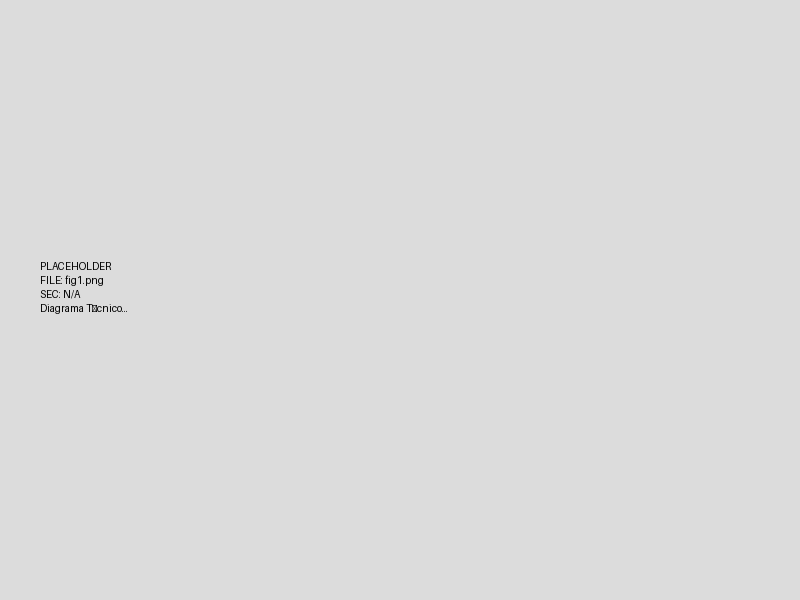
\includegraphics[width=\linewidth]{fig3.png}
\caption{Flujo metodológico general del análisis de factibilidad del sistema redundante VENESAT-2}
\label{fig:flujo_metodologia}
\end{figure}

La Figura 3 ilustra el flujo integrado de la metodología, donde se aprecia la interacción entre balance de enlace, modelado de propagación y análisis FMEA. Este enfoque holístico, aunque más demandante computacionalmente, permite obtener conclusiones con mayor grado de confianza que análisis aislados. No obstante, cabe matizar que toda simulación posee limitaciones inherentes; por ello, los resultados aquí obtenidos se interpretarán con prudencia y se validarán contra mediciones de campo en fases posteriores del proyecto.